\documentclass{article}
\usepackage[utf8]{inputenc}
\usepackage{graphicx}
\usepackage[margin=1in]{geometry}
\usepackage[dvipsnames]{xcolor}
\usepackage{url}
\usepackage{hyperref}
\usepackage{subcaption}
\usepackage[numbers]{natbib} % for numeric references

\setlength{\columnsep}{0.25in}
\renewcommand{\topfraction}{0.9}
\renewcommand{\bottomfraction}{0.9}
\renewcommand{\textfraction}{0.05}
\setlength{\textfloatsep}{8pt}
\setlength{\floatsep}{6pt}
\setlength{\abovecaptionskip}{4pt}

\begin{document}

\begin{titlepage}
    \begin{center}
        \includegraphics[width=10cm]
        %Changed to 10 cause it looks better ;) 
        {figures/MSP-logo.jpg} 
        \vspace{1cm}
        
        \textbf{\LARGE How Does COVID-19 Case Fatality Vary by Age, Sex and Ethnicity, and How Did It Change Over Time?}\\
        \textbf{\LARGE An analysis of the CDC COVID-19 Case Surveillance Public Use Data}
        
        \vspace{1.5cm}
        
        \textbf{\Large Julian Lenders (I6404793)}
        
        \vfill
        
        \large Date: \today
        
    \end{center}
\end{titlepage}

\twocolumn[
\section*{Introduction}
Since the first cases of COVID-19 were reported in early 2020, it has been clear that the risk of dying from the disease is far from uniform. Older people were identified early as a high-risk group \cite{death_by_age}, and men were reported to die more often than women \cite{peckham}. Ethnic differences are harder to interpret, because groups differ in age structure, access to care and underlying health, and it is less well documented how all these risks shifted as testing, treatment, vaccination and variants changed.

This report therefore addresses the question: how does COVID-19 case fatality vary between patients (age, sex, ethnicity), and how did these patterns change over time? Case fatality was expected to rise steeply with age, to be higher in men than in women, and to decline over time. Using the CDC case surveillance data \cite{cdc}, case fatality is estimated with confidence intervals, compared between sexes within age groups, age-standardized across ethnic groups, and followed monthly for four age bands. Comorbidities and immunocompromise cannot be analyzed, because the public dataset does not contain them.

Case fatality is defined as deaths divided by cases with a known outcome; cases with an unknown death status are excluded. It is not the infection fatality rate, whose denominator is all infections rather than only diagnosed cases with a recorded outcome.
%Brief introduction about the topic, phrase the scientific question and place it in a broader context

%changed to two columns as compared to the template, again, because it looks better ;)
\vspace{16pt}
]

\section*{Data sample}
The analysis is based on the COVID-19 Case Surveillance Public Use Data dataset from the Centers for Disease Control and Prevention (CDC) \cite{cdc}, a de-identified file of 106,219,500 cases (about 14 GB as CSV) covering 2020 to 2024. Five out of the twelve available variables were used: earliest case date (combined per month), sex, age group (10-year bands), race/ethnicity, and death status (yes, no, or unknown).

The dataset is not a random sample of all infections. Only 34,071,247 cases (32.1\%) have a known death status, and this share declines from 39\% in 2020 to 24\% in 2024 (Figure~\ref{fig:quality}a). In addition, several jurisdictions stopped reporting or reported only partially from late 2021 onward (Figure~\ref{fig:quality}b). The public file contains no geographic variable, so these jurisdictions could not be excluded.


\section*{Methods}
The raw file was too large to load into memory and was therefore processed in Python in chunks of 5 million rows. Spellings of unknown were mapped to one label, dates outside 2019--2026 were marked invalid, and row counts were verified per chunk and in total. Each chunk was cleaned and counted per combination of month, sex, age group, ethnicity and death status, which reduced 106.2 million rows to 30,768 aggregated rows. The case fatality rate (known outcomes only) is given per group with a 95\% Wilson confidence interval; groups or months with fewer than 100 known outcomes are not shown. Male-versus-female odds ratios (Woolf 95\% confidence interval) were computed within each age group. Ethnic groups were directly age-standardized: age-specific rates of each group were weighted by the age distribution of all known-outcome cases combined. The monthly case fatality rate was followed for four age bands (0--39, 40--59, 60--79 and 80+ years).

\begin{figure}[h!]
  \centering
  \begin{subfigure}[b]{\linewidth}
    \centering
    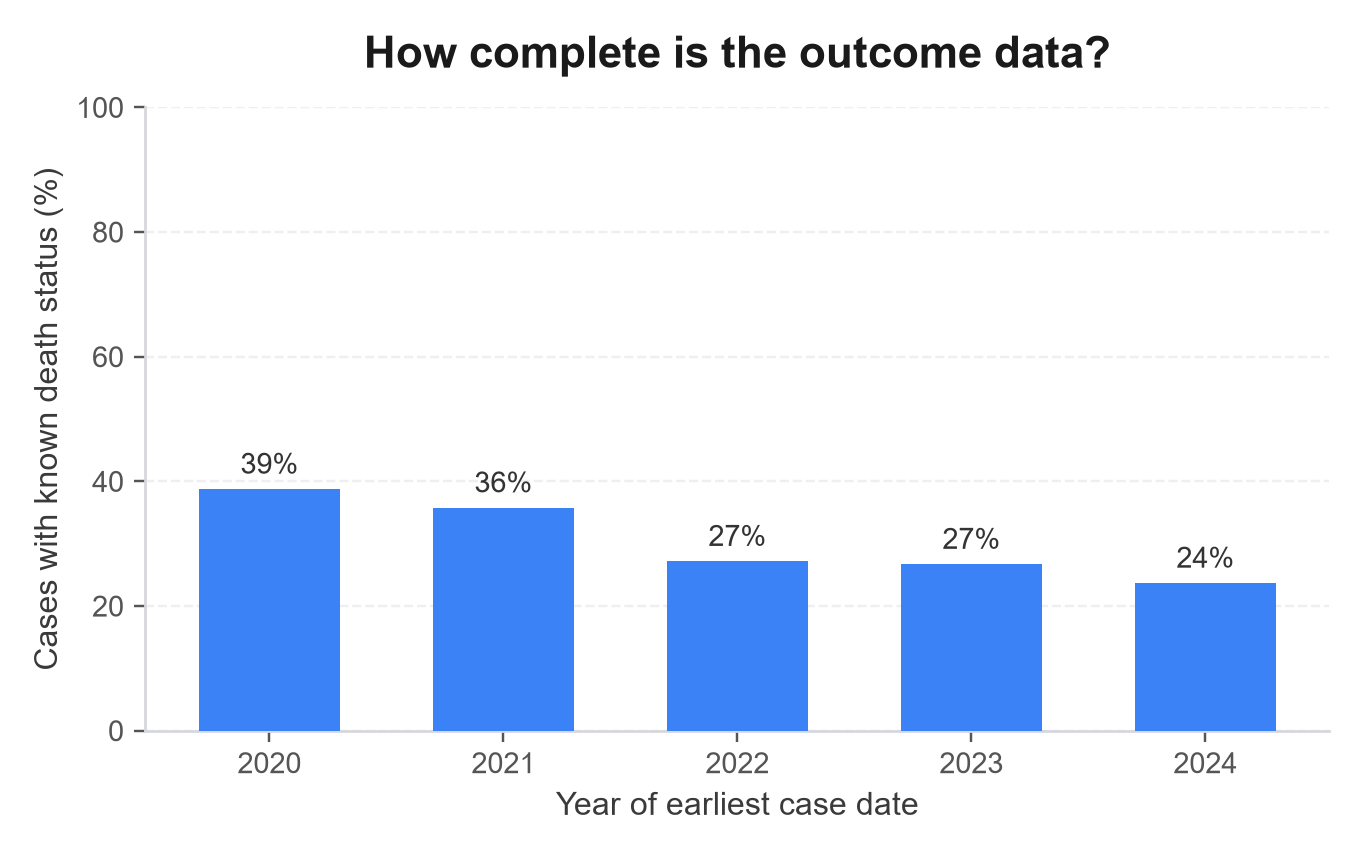
\includegraphics[width=0.88\linewidth]{figures/fig1_missingness.png}
    \caption{}\label{fig:quality-a}
  \end{subfigure}\\[4pt]
  \begin{subfigure}[b]{\linewidth}
    \centering
    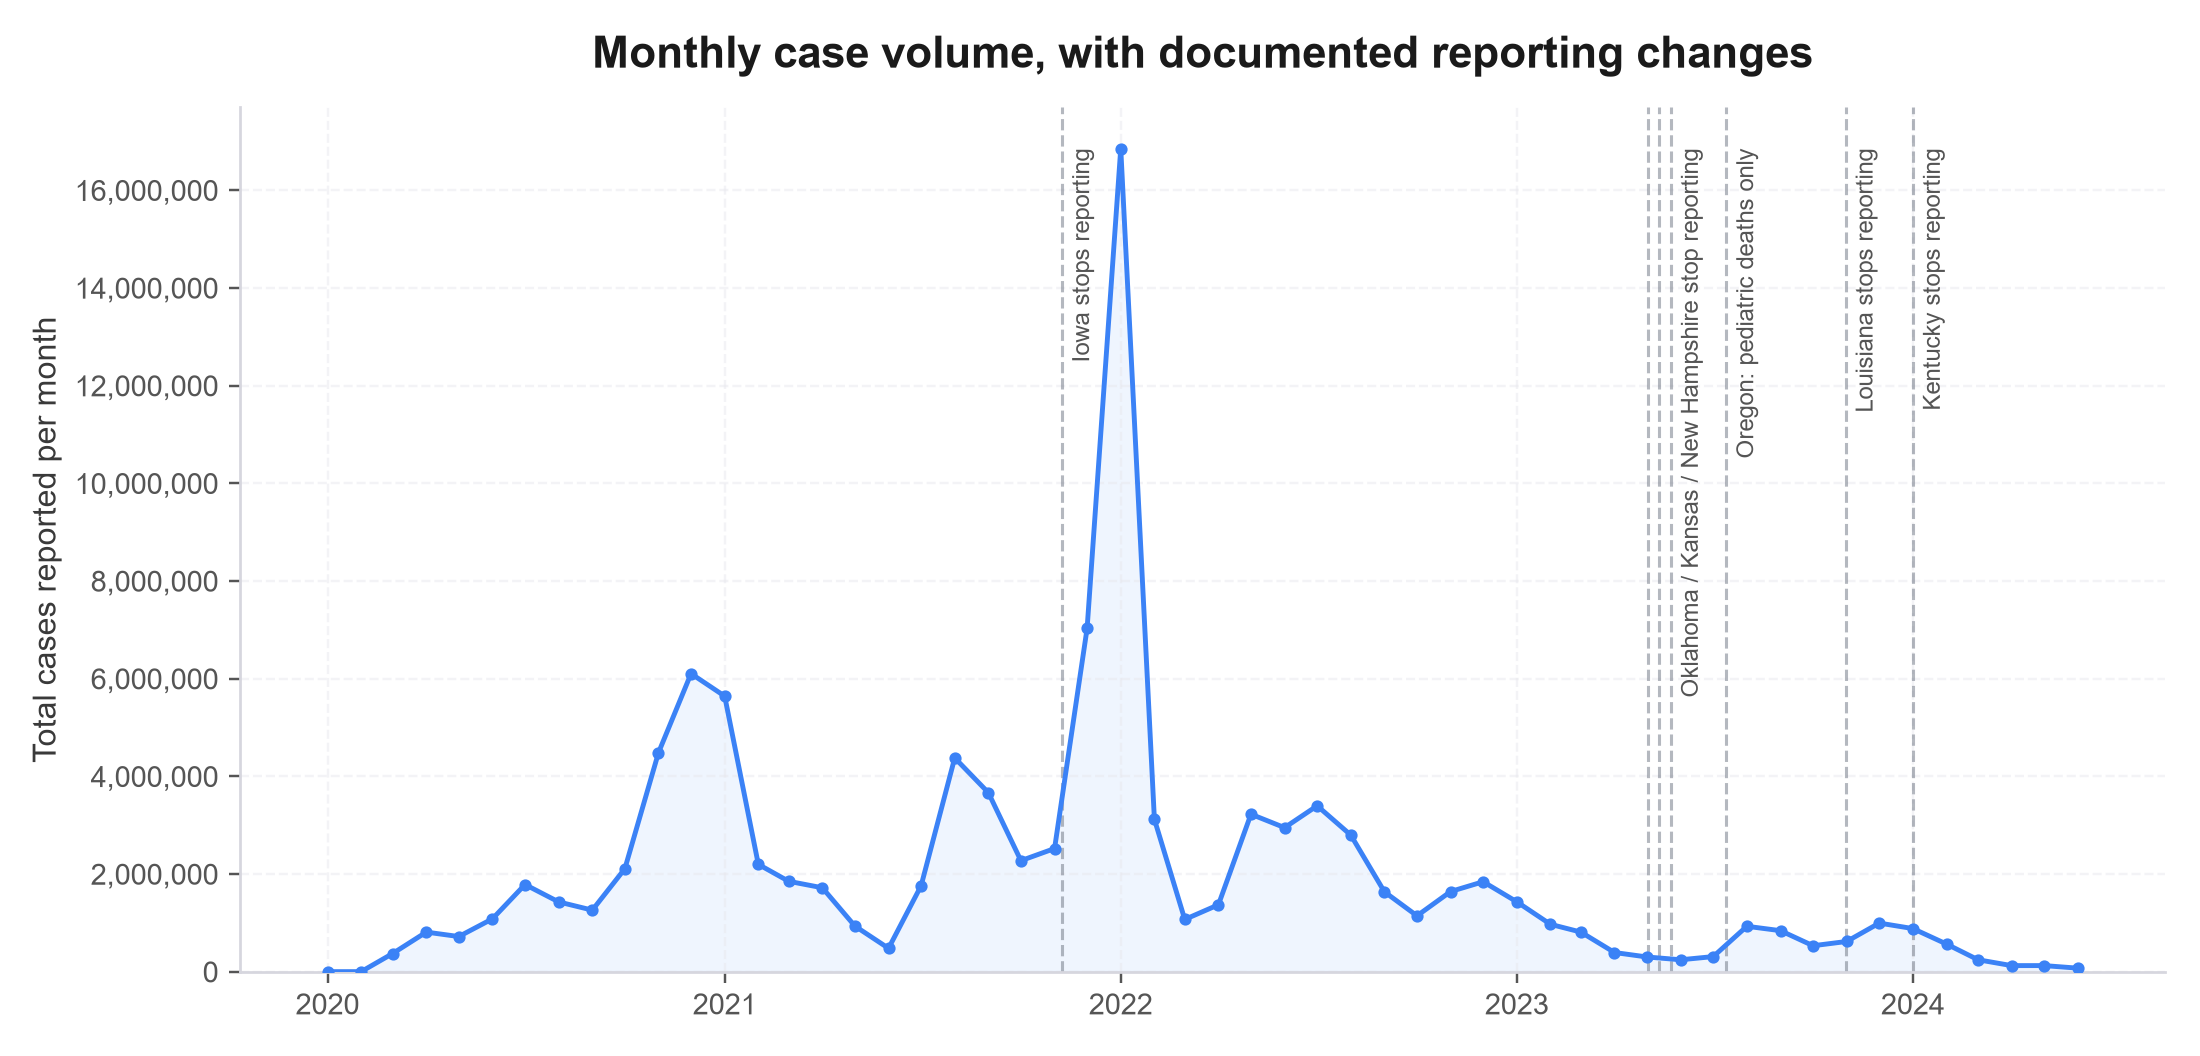
\includegraphics[width=0.88\linewidth]{figures/fig5_reporting_changes.png}
    \caption{}\label{fig:quality-b}
  \end{subfigure}
  \caption{\small Data quality checks. (a) Share of cases with a known outcome per year. (b) Monthly case volume with documented reporting changes.}
  \label{fig:quality}
\end{figure}

\clearpage
\section*{Results and discussion}
\textbf{Age and sex.} Case fatality rises steeply with age (Figure~\ref{fig:main}a). It stays below 3\% in both sexes until age 60 and then climbs to about 6\% in men and 4\% in women at 60 to 69, about 13\% and 9\% at 70 to 79, and about 28\% and 21\% at 80 years and older. Men have a higher case fatality rate than women in every age group. Within age groups, the odds ratio of death for men versus women is about 2 between ages 20 and 59 (maximum odds ratio 2.04, 95\% confidence interval 2.00--2.08, age group 40--49), falls to 1.73 at 60 to 69 and narrows to about 1.4 in the oldest group, although the absolute gap is largest there (about 7 percentage points). Comorbidities were not available, so the cause of the sex difference is not established.

\textbf{Ethnicity.} Crude case fatality ranges from about 2.4\% (multiple/other) to about 4.8\% (Native Hawaiian/Other Pacific Islander; Figure~\ref{fig:main}b). After age standardization, White patients (on average older) fall from about 3.6\% to about 3.0\%, whereas other groups rise, e.g. Hispanic/Latino (3.3\% to 5.4\%), Asian (3.9\% to 5.7\%) and Native Hawaiian/Other Pacific Islander patients (4.8\% to 7.5\%), about 2.5 times the White value. Access to care, comorbidities and calendar time are not adjusted for, so these differences should not be interpreted causally.


\begin{figure}[h!]
  \centering
  \begin{subfigure}[b]{\linewidth}
    \centering
    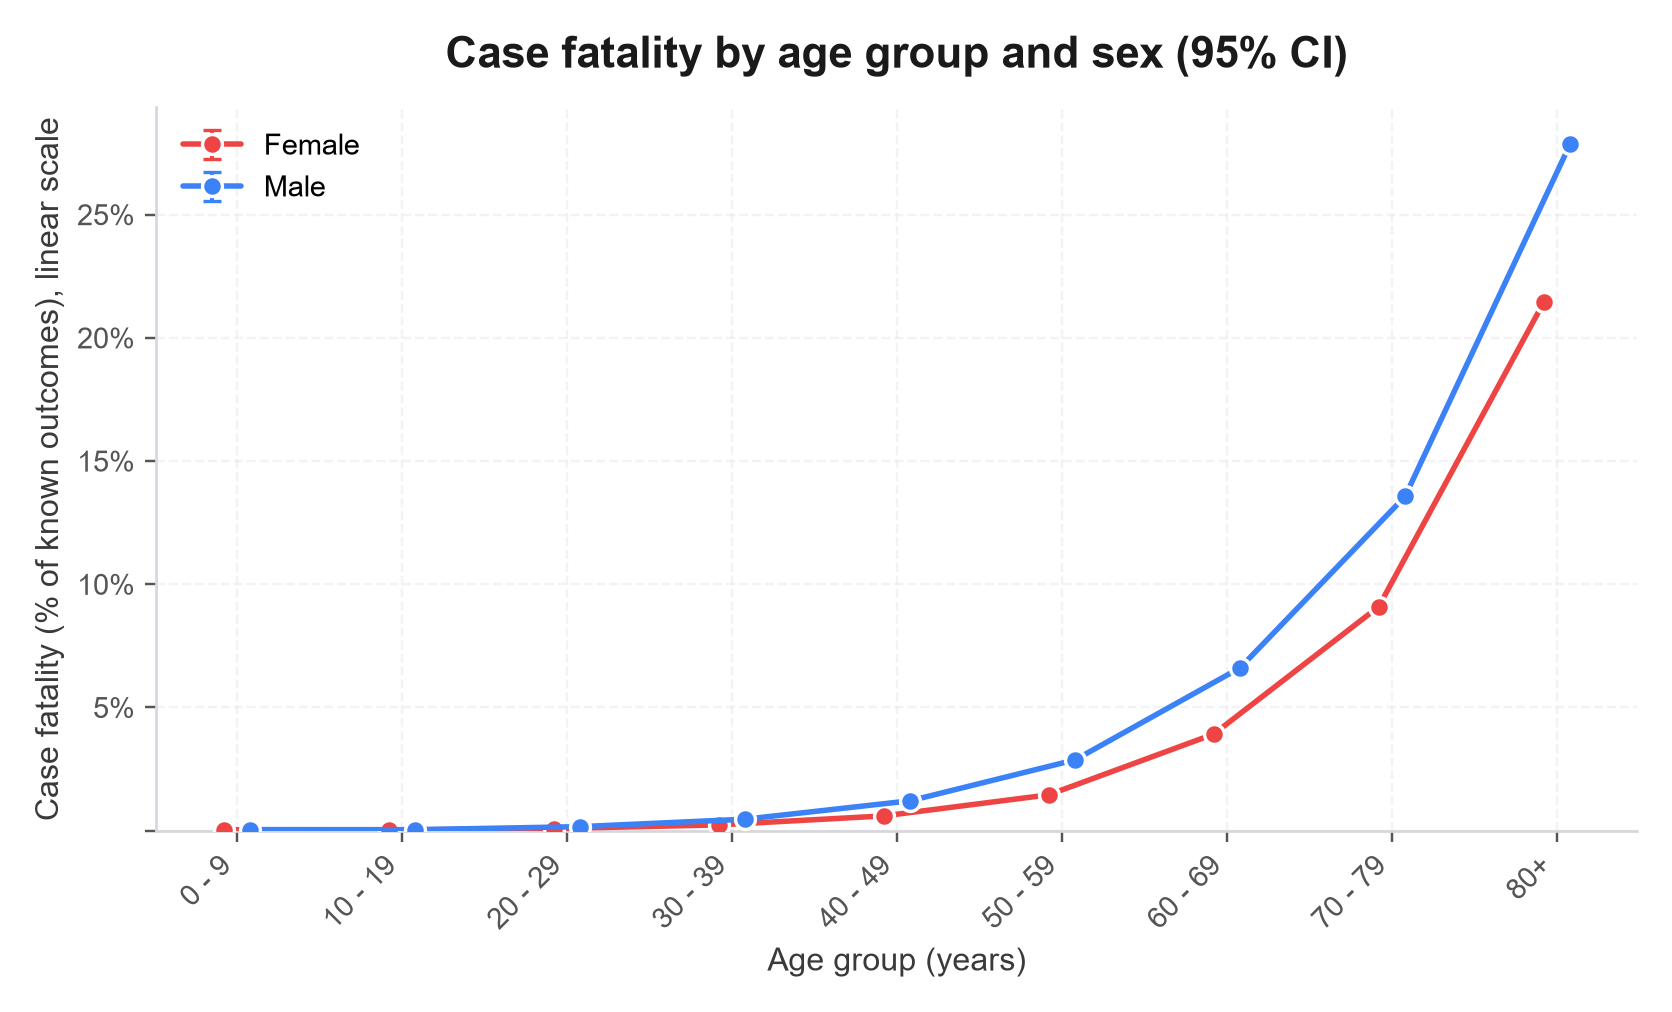
\includegraphics[width=0.80\linewidth]{figures/fig2_age_sex_linear.png}
    \caption{}\label{fig:main-a}
  \end{subfigure}\\[4pt]
  \begin{subfigure}[b]{\linewidth}
    \centering
    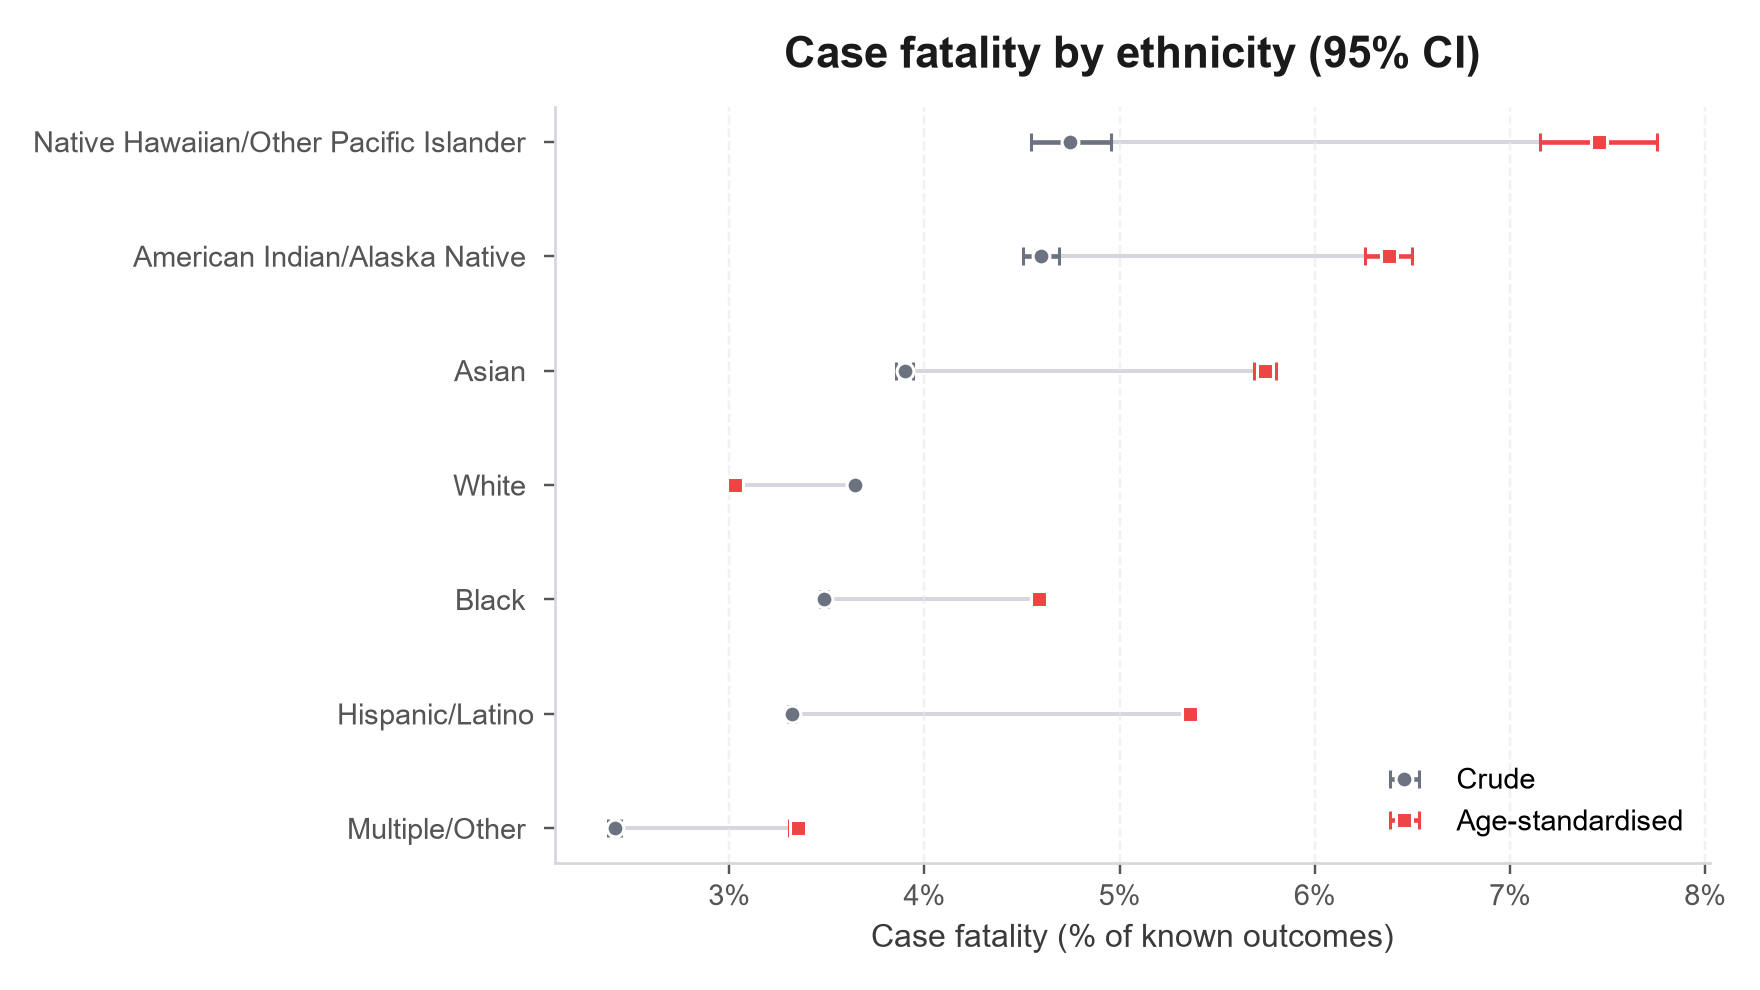
\includegraphics[width=0.80\linewidth]{figures/fig3_ethnicity.png}
    \caption{}\label{fig:main-b}
  \end{subfigure}
  \caption{\small (a) Case fatality rate by age group and sex. (b) Crude and age-standardized case fatality rate by ethnicity. Error bars: 95\% confidence intervals (smaller than the markers in (a)).}
  \label{fig:main}
\end{figure}

\textbf{Time.} The monthly case fatality rate of the 80+ band fell from about 68\% in early 2020 to about 10\% during 2023 and about 8\% in early 2024 (Figure~\ref{fig:time}). The 60--79 band fell from about 48\% in early 2020 to about 3\% in 2023, whereas the 0--39 and 40--59 bands stay below 5\% from mid-2020 onward and are close to zero on this scale. A pronounced step occurred in spring 2022, after the January 2022 case peak (Figure~\ref{fig:quality}b), when the 80+ band dropped from about 22\% to 9\%. This is consistent with vaccination, treatment, variants, prior immunity and more mild cases, but the data cannot separate these effects. Early 2020 values are likely inflated because testing was limited to severe cases, and the fall in the final months may partly reflect incomplete reporting.

Overall, the figures support all three of the original expectations: case fatality rises steeply with age, is higher in men than in women at every age, and fell strongly over time, although the causes of this fall cannot be separated. Differences between ethnic groups remain after age standardization, but access to care and underlying health are not accounted for. These factors are therefore clearly associated with case fatality, but the data do not show that they cause it.

\textbf{Limitations.} 68\% of cases have no recorded outcome, which may bias the case fatality rate in either direction, only age is adjusted for, and several jurisdictions stopped reporting before the data end in mid-2024.

\begin{figure}[h!]
  \centering
  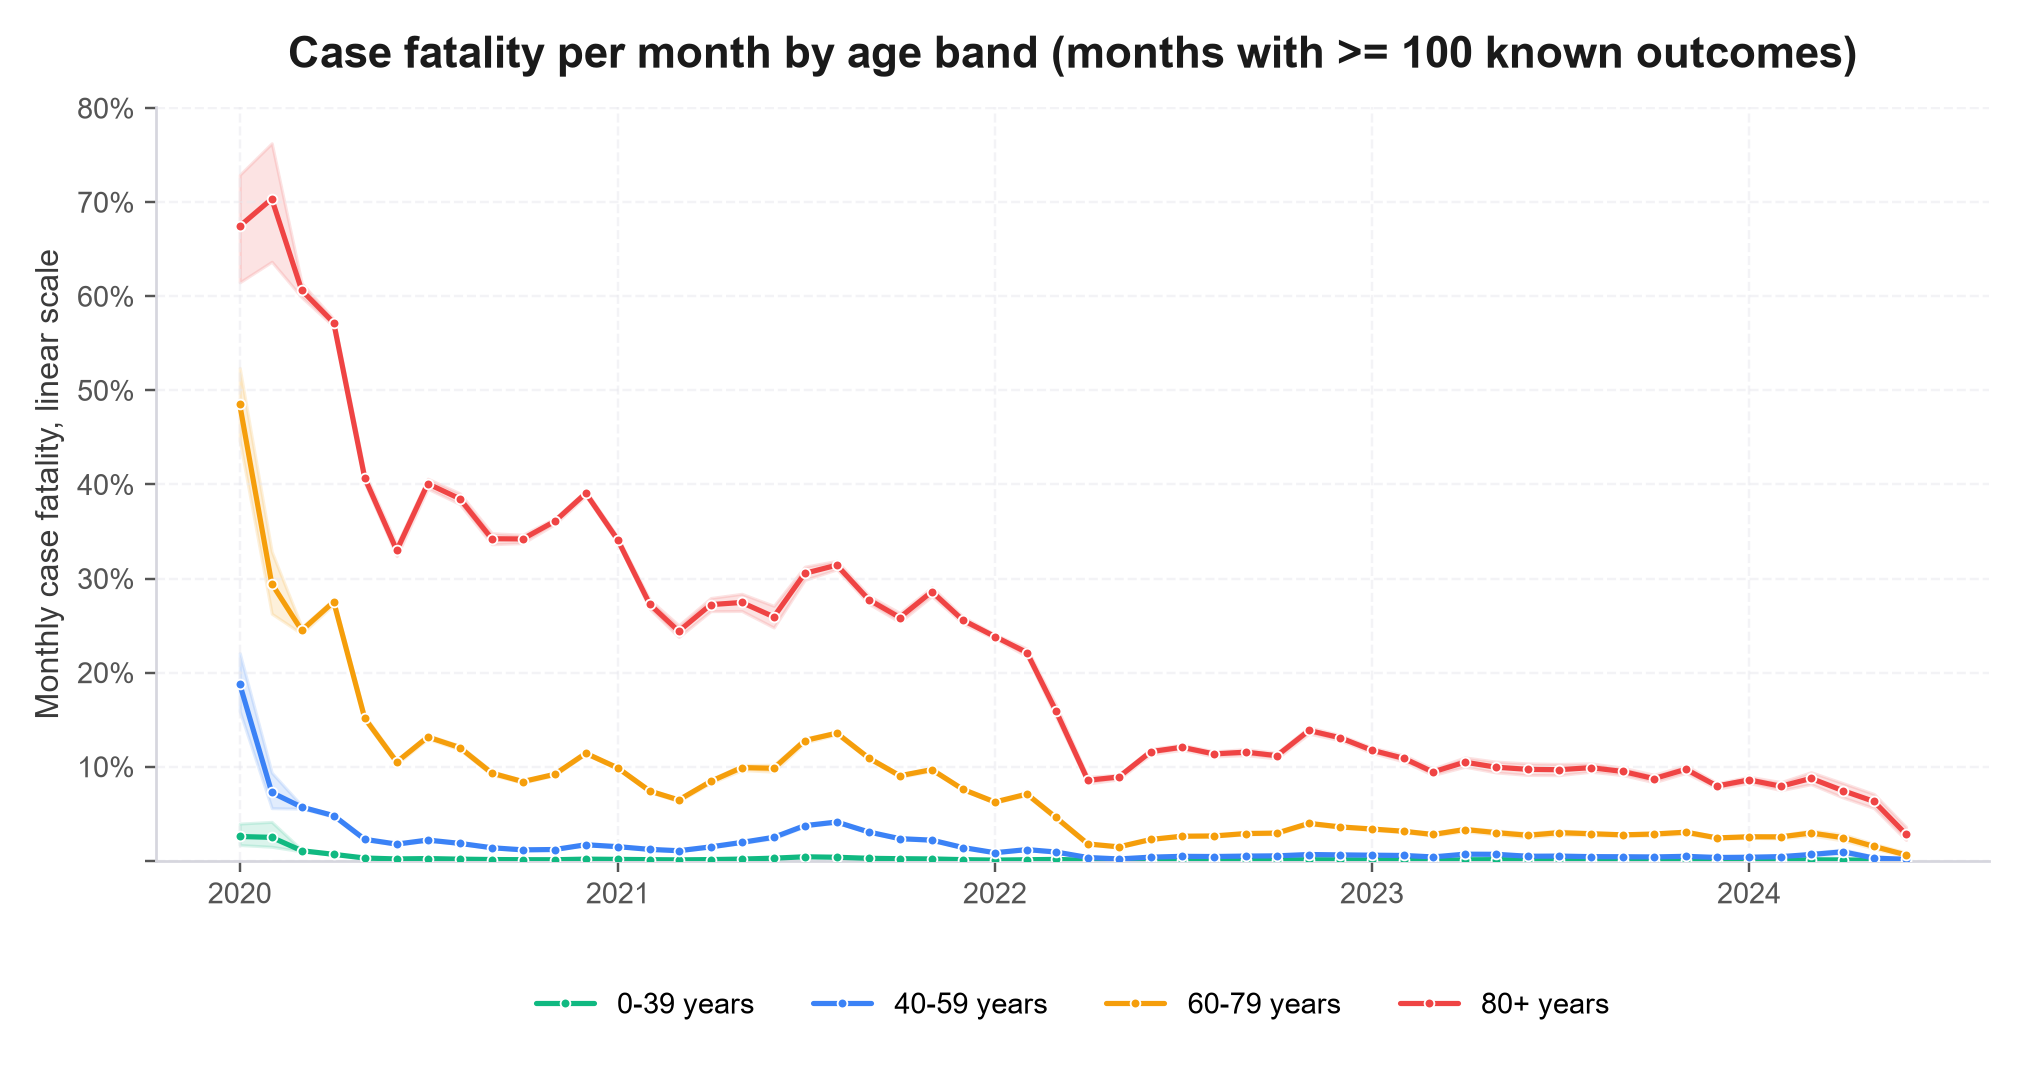
\includegraphics[width=\linewidth]{figures/fig4_monthly_age_linear.png}
  \caption{\small Monthly case fatality rate by age band (linear scale), months with at least 100 known outcomes; shaded bands: 95\% confidence intervals.}
  \label{fig:time}
\end{figure}

\onecolumn
\newpage
\begin{thebibliography}{9}

\bibitem{cdc}
Centers for Disease Control and Prevention. (n.d.). \textit{COVID-19 case surveillance public use data} [Data set]. Retrieved on the 4th of October 2026, from:
\href{https://data.cdc.gov/Case-Surveillance/COVID-19-Case-Surveillance-Public-Use-Data/vbim-akqf/about_data}{https://data.cdc.gov/Case-Surveillance/COVID-19-Case-Surveillance-Public-Use-Data/vbim-akqf/about\_data}

\bibitem{death_by_age}
Glynn, J. R., \& Moss, P. A. H. (2020). Systematic analysis of infectious disease outcomes by age shows lowest severity in school-age children. \textit{Scientific Data, 7}(1), 329. 
\href{https://doi.org/10.1038/s41597-020-00668-y}{https://doi.org/10.1038/s41597-020-00668-y}

\bibitem{peckham}
Peckham, H., de Gruijter, N. M., Raine, C., Radziszewska, A., Ciurtin, C., Wedderburn, L. R., Rosser, E. C., Webb, K., \& Deakin, C. T. (2020). Male sex identified by global COVID-19 meta-analysis as a risk factor for death and ITU admission. \textit{Nature Communications, 11}(1), 6317.
\href{https://doi.org/10.1038/s41467-020-19741-6}{https://doi.org/10.1038/s41467-020-19741-6}

\end{thebibliography}
\end{document}